\section{Cropflip}

\subsection{Descripción}
La imagen destino del filtro consiste en invertir verticalmente (flip) un recorte (crop) de la imagen fuente a partir de offsets dados como parámetro. El ancho y alto en píxeles de la imagen destino también se pasa como parámetros.
La descripción matemática está dada por la fórmula:

$$ O_{i,\ j}^{k}=I_{tamy+offsety-i-1, \ \ offsetx+j}^{k} $$

Donde el 'crop' de la imagen input corresponde con los píxeles del tipo:

$$
I_{offsety+i, \ \ offsetx+j}^{k}
\qquad \text{con} \quad 0 \leq i < tamy \ \ \ 0 \leq j < tamx
$$

\begin{table}[h]
\centering
\mem
\begin{tabular}{l|c|c|c|c|c|c|l}
 & \multicolumn{1}{l|}{}      & \multicolumn{1}{l|}{}       & \multicolumn{1}{l|}{}       & \multicolumn{1}{l|}{}       & \multicolumn{1}{l|}{}       & \multicolumn{1}{l|}{}      &  \\ \hline
 & \cellcolor[HTML]{FFCB2F}$I_{30}$ & \cellcolor[HTML]{FFCB2F}$I_{31}$  & \cellcolor[HTML]{FD6864}$I_{32}$  & \cellcolor[HTML]{FD6864}$I_{33}$  & \cellcolor[HTML]{FD6864}$I_{34}$  & \cellcolor[HTML]{FD6864}$I_{35}$ &  \\ \hline
 & \cellcolor[HTML]{FFCB2F}$I_{24}$ & \cellcolor[HTML]{FFCB2F}$I_{25}$  & \cellcolor[HTML]{FD6864}$I_{26}$  & \cellcolor[HTML]{FD6864}$I_{27}$  & \cellcolor[HTML]{FD6864}$I_{28}$  & \cellcolor[HTML]{FD6864}$I_{29}$ &  \\ \hline
 & \cellcolor[HTML]{FFCB2F}$I_{18}$ & \cellcolor[HTML]{FFCB2F}$I_{19}$ & \cellcolor[HTML]{FD6864}$I_{20}$ & \cellcolor[HTML]{FD6864}$I_{21}$ & \cellcolor[HTML]{FD6864}$I_{22}$  & \cellcolor[HTML]{FD6864}$I_{23}$ &  \\ \hline
 & \cellcolor[HTML]{FFCB2F}$I_{12}$ & \cellcolor[HTML]{FFCB2F}$I_{13}$ & \cellcolor[HTML]{FD6864}$I_{14}$ & \cellcolor[HTML]{FD6864}$I_{15}$ & \cellcolor[HTML]{FD6864}$I_{16}$  & \cellcolor[HTML]{FD6864}$I_{17}$ &  \\ \hline
 & \cellcolor[HTML]{FFCB2F}$I_{6}$ & \cellcolor[HTML]{FFCB2F}$I_{7}$ & \cellcolor[HTML]{FFCB2F}$I_{8}$ & \cellcolor[HTML]{FFCB2F}$I_{9}$ & \cellcolor[HTML]{FFCB2F}$I_{10}$  & \cellcolor[HTML]{FFCB2F}$I_{11}$ &  \\ \hline
 & \cellcolor[HTML]{FFCB2F}$I_{0}$ & \cellcolor[HTML]{FFCB2F}$I_{1}$ & \cellcolor[HTML]{FFCB2F}$I_{2}$ & \cellcolor[HTML]{FFCB2F}$I_{3}$ & \cellcolor[HTML]{FFCB2F}$I_{4}$  & \cellcolor[HTML]{FFCB2F}$I_{5}$ &  \\ \hline
 & \multicolumn{1}{l|}{}      & \multicolumn{1}{l|}{}       & \multicolumn{1}{l|}{}       & \multicolumn{1}{l|}{}       & \multicolumn{1}{l|}{}       & \multicolumn{1}{l|}{}      &
\end{tabular}
\caption{Ilustración de la imagen fuente en memoria. En rojo los píxeles del crop \newline
(offsetx = 2, offsety = 2, tamx = 4, tamy = 4)}
\end{table}

\begin{table}[h]
\centering
\mem
\begin{tabular}{l|c|c|c|c|l}
& \multicolumn{1}{l|}{}       & \multicolumn{1}{l|}{}   & \multicolumn{1}{l|}{}     & \multicolumn{1}{l|}{}      &  \\ \hline
 & \cellcolor[HTML]{FD6864}$I_{14}$ & \cellcolor[HTML]{FD6864}$I_{15}$ & \cellcolor[HTML]{FD6864}$I_{16}$  & \cellcolor[HTML]{FD6864}$I_{17}$ &  \\ \hline
 & \cellcolor[HTML]{FD6864}$I_{20}$ & \cellcolor[HTML]{FD6864}$I_{21}$ & \cellcolor[HTML]{FD6864}$I_{22}$  & \cellcolor[HTML]{FD6864}$I_{23}$ &  \\ \hline
 & \cellcolor[HTML]{FD6864}$I_{26}$  & \cellcolor[HTML]{FD6864}$I_{27}$  & \cellcolor[HTML]{FD6864}$I_{28}$  & \cellcolor[HTML]{FD6864}$I_{29}$ &  \\ \hline
  & \cellcolor[HTML]{FD6864}$I_{32}$ & \cellcolor[HTML]{FD6864}$I_{33}$  & \cellcolor[HTML]{FD6864}$I_{34}$  & \cellcolor[HTML]{FD6864}$I_{35}$ &  \\ \hline
  & \multicolumn{1}{l|}{}       & \multicolumn{1}{l|}{}  & \multicolumn{1}{l|}{}      & \multicolumn{1}{l|}{}      &
\end{tabular}
\caption{Ilustración de la imagen destino en memoria}
\end{table}




No es difícil notar que las filas del crop en la fuente no constituyen una tira contigua de píxeles en memoria, si no que se encuentran distanciadas por el tamaño en bytes de offsetx lo que implica que necesitaremos iterar en dos ciclos anidados para poder procesar el crop.

\subsection{Implementaciones}
Al no involucrar operaciones aritméticas entre componentes de la imagen, las implementaciones del filtro se centran en accesos a memoria. Por lo tanto, las implementaciones solamente difieren en el modo en que se copian y asignan píxeles a la imagen output, radicando en esos métodos nuestro foco de análisis.
\subsubsection{Implementaciones C y SSE}
La implementación C simplemente se trata de recorrer la imagen con una sola variable aplicando pixel a pixel la transformación dada por la fórmula matemática previamente mencionada. Mientras que la implementación correspondiente a SSE recorre la imagen fuente desde la fila superior del recuadro ($I_{32}$ en el cuadro 1) del crop hacia abajo de a 4 píxeles por iteración como indica el siguiente pseudo-código:


\begin{codesnippet}
\begin{verbatim}

temp = src + offsetx*4 +srcRowSize*(offsety+tamy-1)
{Apunta al primer píxel de la esquina superior izq. del crop}
for i = 0 to tamy:
--> for j = 0 to tamx:
-----> xmm0 = [temp]
-----> [dst] = xmm0
-----> dst = dst  + 16
-----> temp =  temp + 16
-----> temp = temp - (dstRowSize + srcRowSize)
{Decrece el ancho de la imagen destino y el de la fuente para apuntar primer pixel de la fila de
abajo a la que procesó}
--> end for
end for

\end{verbatim}
\end{codesnippet}



De esta manera, las lecturas y escrituras en memoria representan $\frac{1}{16} = 0,0625 =  6,25\%$ del total de los accesos a memoria de la implementación C.


\subsubsection{Implementaciones SIMD paralelo en 128 y 256 bits}
Se diferencian de la implementación anterior de SSE en el uso de la mayor cantidad posible de registros \xmm{} (\ymm{} de 256 bits en el caso de las implementaciones de AVX) para las operaciones de transferencia de bloques de píxeles de la imagen fuente a la destino.
\\

Dado que las lecturas y escrituras en memoria de cada registro son independientes entre sí, la ejecución fuera de orden del procesador hace que la transferencia por bloque sea más rápida que la implementación individual (que recorre la imagen con un único registro \xmm{}). Por cuestiones de vecindad espacial de los píxeles en la memoria, los accesos a memoria de cada registro tienen chances particularmente altas de hit en caché, no demorando así las lecturas del resto de los registros.
\\

Recordando que los registros de AVX tienen 32 bytes de capacidad y cada pixel en nuestro formato ocupa 4 bytes, cada registro \ymm{} tendrá capacidad para:

$$ \frac{32 \ bytes}{4 \ \frac{bytes}{px}} = 8 \ px $$

Por lo cual, suponiendo $ tamx \equiv 0 \ (mod \ 8) $ (como es el caso de una imagen de salida de 512x512), tendríamos $\frac{1}{32} = 0,03125 =  3,125\%$ del total de accesos a memoria de la implementación en C.

\subsubsection{Copiado paralelo de vectores}
\label{explicacionCopyN}

La asignación de píxeles se hace llamando a las funciones externas 'copyN_sse' y 'copyN_avx2'\footnote{../entregable/tp2-bundle.v1/codigo/lib} que copian tiras de píxeles de una imagen a otra por bloques de 64/4/1 ó 128/8/1 píxeles (sse y avx2 respectivamente) según sea posible en cada iteración. A modo de ejemplo (los otros casos son análogos), para copiar bloques de 64px (256B) desde la posición indicada por rsi a la indicada por rdi se cargan los valores correspondientes de la siguiente manera:
\newline
\\
\xmm{0} $\leftarrow$ {[rsi]} \\
\xmm{1} $\leftarrow$ {[rsi+16]} \\
... \\
\xmm{14} $\leftarrow$ {[rsi+224]}  \\
\xmm{15} $\leftarrow$ {[rsi+240]} \\
\\
{[rdi]} $\leftarrow$ \xmm{0} \\
{[rdi+16]} $\leftarrow$ \xmm{1} \\
... \\
{[rdi+224]} $\leftarrow$ \xmm{14} \\
{[rdi+240]} $\leftarrow$ \xmm{15} \\

Esta técnica de aplicar por cada iteración operaciones que, comúnmente, se harían en varias se conoce como 'loop unrolling'. Como desventaja frente a la optimización por paralelismo y minimización de branch mispredictions, en códigos de mucho mayor tamaño podría aumentar tan significativamente el tamaño del binario que aumente fuertemente el número de 'cache misses'. En nuestro caso copyN.o (que incluye a 'copyN_sse' y 'copyN_avx2') pesa 3,3 kB y es bastante probable que entre enteramente en caché.
\\

En el caso del filtro Cropflip, las tiras de píxeles corresponden a tiras de tamaño 'tamx' (es decir, al ancho del crop).
\\

\subsection{Experimentos - Rendimiento y análisis}

\subsubsection{Comparación entre implementaciones}

\begin{figure}[h]
\centering
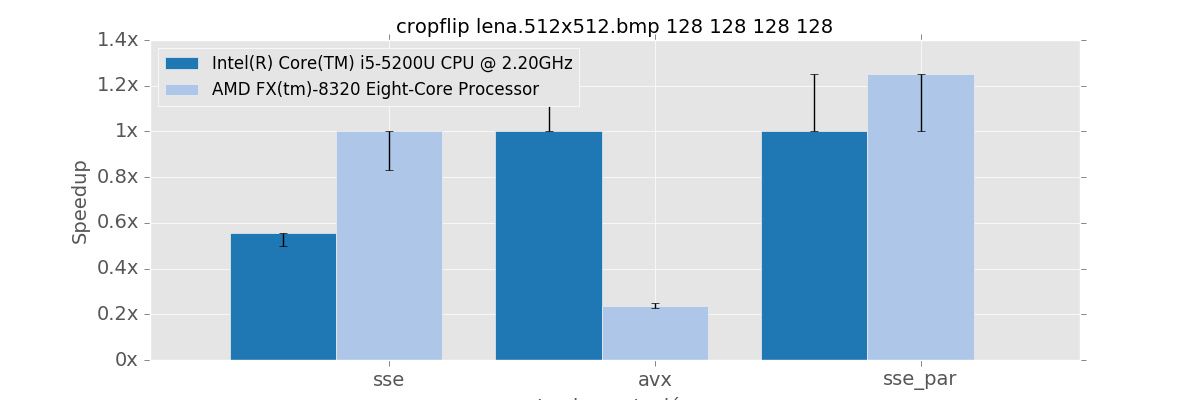
\includegraphics[width=0.90\textwidth]{cropflip-time-speedup}
\caption{Tiempo de ejecución relativo de implementaciones ASM de cropflip contra la implementación C compilada con -O3}
\label{fig:cropflip-time-speedup}
\end{figure}

Algo interesante que nos sucedió fue que, originalmente, al hacer benchmarks con imágenes de 124x124 px, el filtro corría tan rápido que comprometía la fidelidad de la medición en los benchmarks. Así que finalmente optamos por expandir el tamaño de las imágenes de prueba.
\\

A diferencia de los otros dos filtros, donde el procesamiento de imágenes involucra operaciones aritméticas paralelas, la implementación AVX de Cropflip no presenta 'speedup' respecto de las implementaciones de SSE con registros de 128 bits en paralelo. No sólo eso sino que demuestra menor rendimiento que su contraparte de SSE.


Investigando un poco sobre por qué sucedía esto, encontramos que en el Manual de Optimización de Sofware de Intel \footnote{Sección 11.6.2 - "DATA ALIGNMENT FOR INTEL® AVX - Consider 16-Byte Memory Access when Memory is Unaligned"} se sugiere que, para accesos vectorizados a memoria desalineada, el rendimiento de AVX podría ser menor que el de SSE. Lo cual coincide exactamente con nuestro caso.

Sí se presentan entre las dos implementaciones de SSE, donde la diferencia es un poco más fuerte a favor de SSE 'paralela'. Dados los parámetros tales que el recuadro de crop mide 1024x1024 px, en la implementación con loop unrolling alcanza con dieciséis iteraciones procesando 64px en cada una para cubrir cada fila. Mientras que para la versión SSE común hay que recorrer: $\frac{1024 \ \frac{px}{fila}}{8 \ \frac{px}{iteracion}} = 128 \ \frac{iteraciones}{fila}$ .
\\
Sin embargo, la cantidad de iteraciones no refleja el hecho de que aún en ejecución fuera de orden los accesos a memoria siguen siendo individuales, teniendo que 'resecuencializar' las instrucciones para acceder ordenadamente. Podría suponerse que es debido a esto que el speedup no es del orden de magnitud que sugerirían las respectivas iteraciones por fila.
\\
Otra de las razones por las cuales el loop unrolling para copias de memoria no muestra una diferencia tan significativa es porque la microarquitectura Intel Core ejecuta hasta un $load$ y un $store$ de 128 bits por ciclo \footnote{Intel Optimization Manual - 2.4.4.1 - Loads and Stores}. Por lo tanto cargar un \ymm{} toma dos ciclos de ejecución, y termina siendo lo mismo fetchear dos cargas/descargas de 128b a una de 256b si se stallea el pipeline un ciclo más hasta liberar el puerto. Aún así, sigue entre las bondades del loop unrolling el poder coordinar por ejecución fuera de orden el $store$ anterior con el último $load$ en un único ciclo, siguiendo las características mencionadas anteriormente de Intel Core.
\\
A esto último adicionamos el hecho de que el direccionamiento con $base$-$indice$-$offset$ tiene una latencia de 7 ciclos en AVX2 versus los 5 de SSE (si $offset+base > 2048$, 6 ciclos)\footnote{Intel Optimization Manual - Table 2-19. Effect of Addressing Modes on Load Latency}, lo cual tiene especial importancia en nuestro TP porque es el tipo de direccionamiento habitual en el procesamiento de imágenes.
\\

Como habíamos anticipado al hablar del loop unrolling en SSE, el tamaño del binario no es lo suficientemente grande como para no poder ser cacheado eficientemente. La vecindad espacial de las tiras de píxeles también colaboran para que el hitrate se mantenga alto aún cuando las filas del crop no son contiguas en memoria como comentamos en la descripción.
\\

Es notable como el procesador de AMD es el que corre mas lento la implementación AVX (comportamiento que no vimos en las implementaciones AVX de otros filtros). Suponemos que puede deberse a un mal rendimiento de la implementación de copia a los registros \ymm{}.

\begin{figure}[H]
\centering
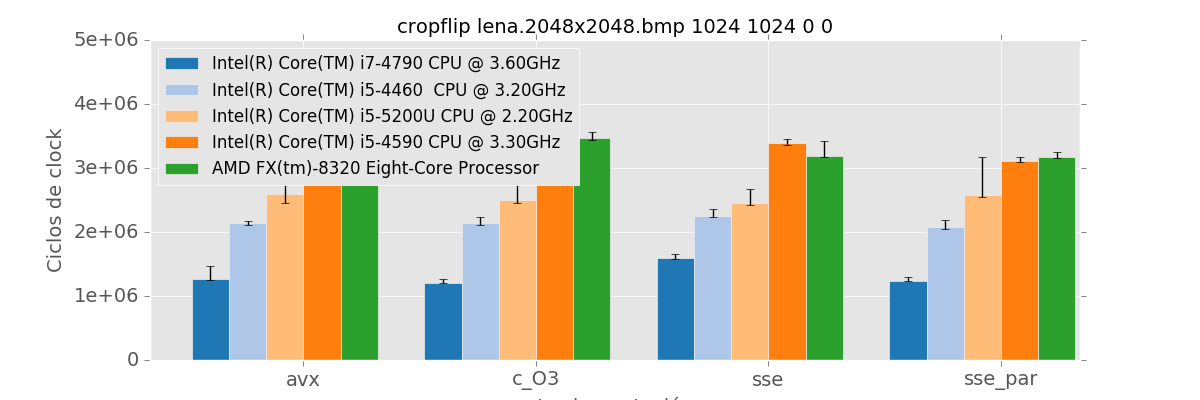
\includegraphics[width=0.90\textwidth]{cropflip-cycles}
\label{fig:cropflip-cycles}
\caption{Ciclos de clock del timestamp counter durante la ejecución del filtro cropflip}
\end{figure}

En este gráfico se nota un poco cómo el techo de los 128 bits por ciclo hacen que el filtro Cropflip, que se basa casi completamente en operaciones $memcpy$, tenga rendimientos homogéneos entre sus implementaciones (salvando algunas diferencias puntuales ya mencionadas). Cuando testeábamos con imágenes más pequelas, curiosamente, el hitrate alto del loop unrolling sobre tiras cortas hacía que resalten un poco más sus puntos fuertes (particularmente paralelismo, no tanto minimizar branch mispredictions como veremos más adelante) a pesar del hecho de que los accesos a memoria son individuales y no pueden solaparse. Al agrandar los tamaños de las imágenes, este efecto fue considerablemente menos masivo.
\\

Pudimos corrobar que no es casualidad que el rendimiento de la implementación en C@-$O3$ sea similar al de las implementaciones SSE utilizando GDB para constrastar dumps del código compilado y comprobando que vectorizaba con operaciones SSE como se muestra a continuación:
\\

\begin{lstlisting}

  >Version usada de GDB: 7.7.1
  >Version usada de GCC: 4.8.4 (cflags: -O3 -Wall -ggdb -std=c99 -pedantic -m64)


  Dump of assembler code for function cropflip_c_o3:
  [...]
  $0x0000000000403eb7$ <+$231$>:	movdqu xmm0,XMMWORD PTR [rcx+rax*1]
  $0x0000000000403ebc$ <+$236$>:	add    edx,0x1
  $0x0000000000403ebf$ <+$239$>:	movdqu XMMWORD PTR [rsi+rax*1],xmm0
  $0x0000000000403ec4$ <+$244$>:	add    rax,0x10
  $0x0000000000403ec8$ <+$248$>:	cmp    edx,ebx
  $0x0000000000403eca$ <+$250$>:	jb     0x403eb7 <cropflip_c_o3+231>
  [...]

\end{lstlisting}

Para testear sobre las versiones actuales (al momento de realizar los tests) de GDB/GCC, corrimos con las versiones 7.11 y 5.3.1 respectivamente de cada herramienta. Al margen de haber diferencias en el resto del código (quizás optimizaciones de compilador que no estén en nuestra versión de SSE, justificando la muy pequeña diferencia vista anteriormente), el dump desensablaba el mismo ciclo.
\\

A modo comparativo también incluimos el análisis de rendimiento entre las diversas optimizaciones para la implementación de C, donde vemos que los estimativos que hicimos anteriormente realmente (respecto de la cantidad de accesos a memoria para C) eran más bien una simplificación 'grosso modo' sin tener en cuenta que la relación C(O$0$)/compilado en ASM no es tan directa como pretendíamos.
\\

\begin{figure}[H]
\centering
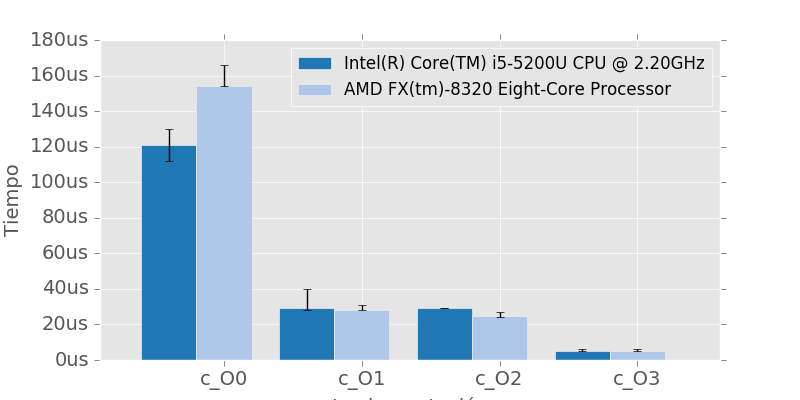
\includegraphics[width=0.90\textwidth]{cropflip-c-time}
\label{fig:cropflip-c-time}
\caption{Tiempo de ejecución de la implementación C del filtro cropflip compilada con distintos optimizaciones}
\end{figure}

También es remarcable el salto en rendimiento se produce entre versiones de C con optimización menor a -O3, donde bajan del rango de 0.3-0.5 milisegundos para las implementaciones C-O1/C-O2 a menos de 0.1 milisegundo (100 microsegundos)  para las C-03, lo cual seguramente tenga que ver con el uso de accesos vectorizados y alguna otra optimización del compilador no tan significativa como para diferenciarse de la implementación SSE.
Más a simple vista, se puede ver el pobre rendimiento de C sin optimizar, entre 12 y 20 veces más lento que la implementación de 03.
\\

\subsubsection{Caché misses}

Volviendo a la idea de la importancia del copiado de memoria en el filtro Cropflip, resulta inherentemente crucial entonces un funcionamiento favorable de la caché para que estos accesos no stalleen el procesamiento. Por ese motivo, en esta sección analizaremos un poco precisamente ese funcionamiento a partir de gráficos generados sobre benchmarks en un procesador con características de 8M de caché, en función del ancho y alto en píxeles de la imagen input.

\begin{figure}[H]
\centering
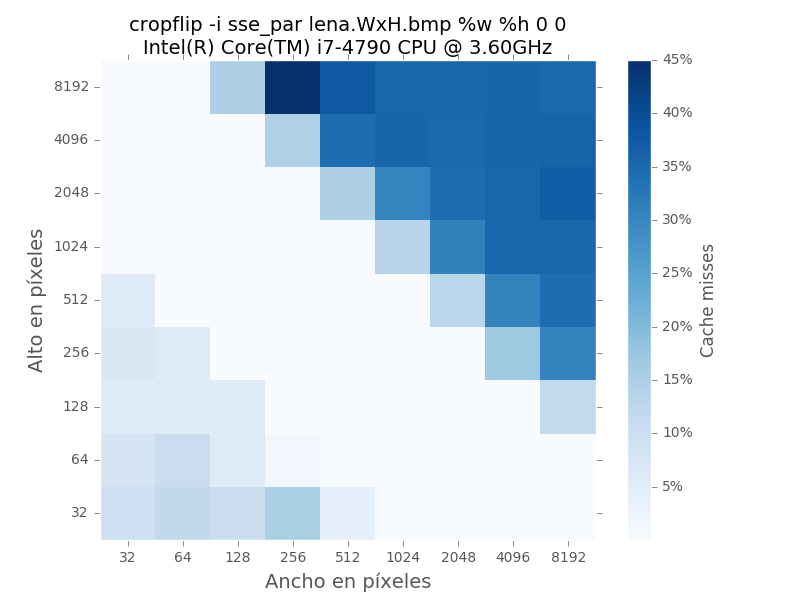
\includegraphics[width=0.7\textwidth]{cropflip-cache-map-sse-par-gflan-MS-7817}
\caption{Porcentaje de misses de la cache en función del tamaño durante la ejecución del filtro cropflip, copiando e invirtiendo la imagen entera en el procesador mencionado anteriormente}
\label{fig:cropflip-cache-map-sse_par-gflan-MS-7817}
\end{figure}


Observamos que, como realizamos las corridas con la caché en caliente y gracias a la vecindad temporal, cuando el tamaño en bytes de la imagen es menor al de la caché el hitrate se mantiene cerca del 100\%. Cuando la imagen ya no entra en caché se termina desplazando a sí misma durante la ejecución y la cantidad de misses sube hasta cerca del 40\%.

\begin{figure}[H]
\centering
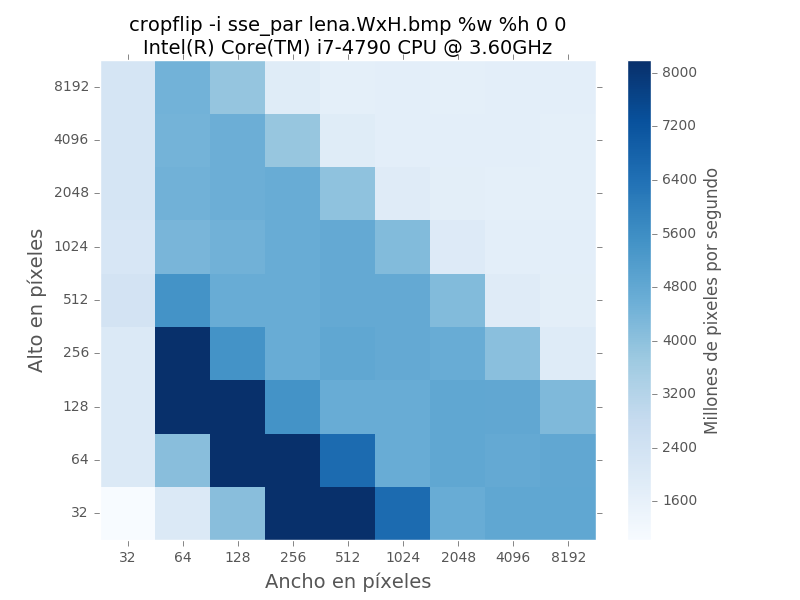
\includegraphics[width=0.7\textwidth]{cropflip-time-rel-map-sse-par-gflan-MS-7817}
\caption{Millones de píxeles procesados por segundo en función del tamaño durante la ejecución del filtro cropflip, copiando e invirtiendo la imagen entera, en un procesador con 8MB de caché L3 y 256kB de caché L2 por núcleo}
\label{fig:cropflip-tame-rel-map-sse_par-gflan-MS-7817}
\end{figure}

En este gráfico podemos observar cómo cuando la imagen ya no entra en caché el throughput baja a menos de la mitad, ya que el procesador se queda esperando a la memoria mas de la mitad del tiempo.

También observamos una segunda franja cuando la imagen ocupa menos de 256kB, que corresponde al tamaño de la caché L2. Es interesante ver la diferencia de rendimiento entre ambas caches, ya que podemos procesar el doble de rápido cuando todos los accesos son a L2.

Cuando la imagen tiene poco ancho el procesamiento se ve interrumpido muy seguido por la lógica de cambio de linea, y el rendimiento se ve afectado.

\subsubsection{Observación sobre las predicciones de saltos}

\begin{figure}[H]
\centering
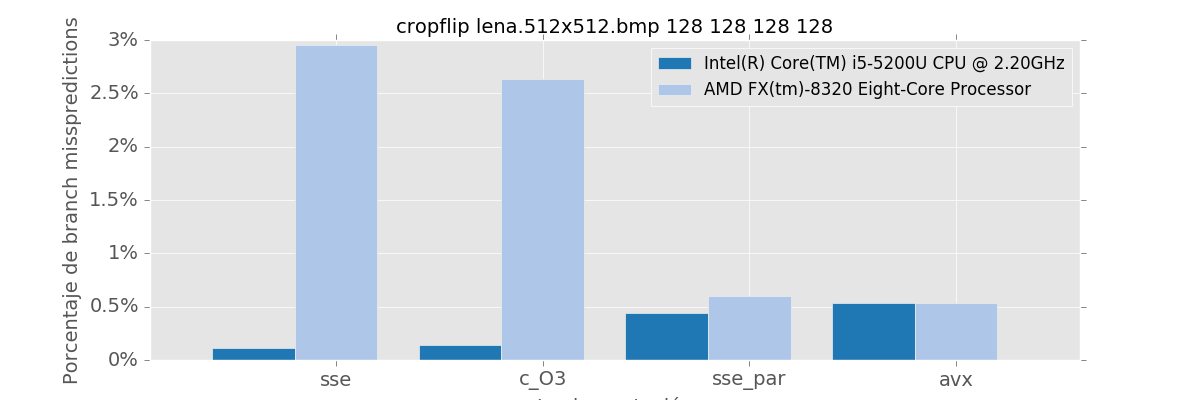
\includegraphics[width=0.90\textwidth]{cropflip-branch-misses}
\label{fig:cropflip-branch-misses}
\end{figure}

En este gráfico se puede apreciar algo bastante curioso: mientras que para algunos procesadores el loop unrolling minimizó muy efectivamente el porcentaje de branch mispredictions en las implementaciones de AVX y de SSE en paralelo frente a las implementaciones que procesan con un único vector (ya vimos que la implementación en C con optimización O3 también usa un registro XMM para los accesos a memoria), para otros significó un retroceso.

\ Esto resulta particularmente contraintuitivo si tenemos en cuenta que en teoría minimizar iteraciones parecería implicar minimizar predicciones y por lo tanto penalidades. Sin embargo esto se puede deber a que, en cada ciclo, se requiere evaluar si la cantidad restante de píxeles para copiar es mayor a  64/4/1 ó 128/8/1 píxeles para poder saltar a cada subrutina. Resultando así contraproducente desde este punto de vista dicha implementación.
